\section{Analysis and Results: How do Machine Learning Methods Perform at Forecasting Inflation?} \label{sec:analysis}

\subsection{Overall Results — Forecasting Inflation} \label{sec:analysis_results}

The results of the forecasting exercise are shown in Figure \ref{fig:cpi}, which includes the one-month ahead forecasts for each model, RF, AR, and Lasso respectively, as well as the out-turn CPI series. A simple visual inspection reveals a number of points. In general, we see that all three models reasonably track the out-turn series. The Lasso overreacts to the negative Covid shock and slightly underreacts to the following inflation during 2021/22.

\begin{figure}[H]
    \centering
    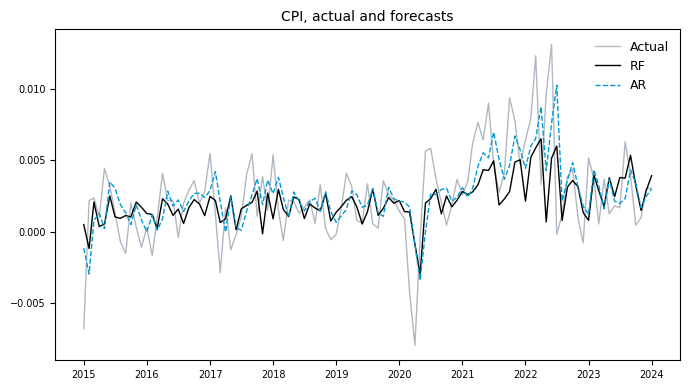
\includegraphics[width=1\linewidth]{figures/forecasts.png}
    \vspace{-30pt}
    \caption{CPI change, actual and forecasts, 1960-2024.}
    \label{fig:forecasts} 
\end{figure}

In assessing the efficacy of various inflation forecasting models over distinct periods characterised by differing economic conditions, I rely on three measures of forecasting error per Equation \ref{eq:errors}: RMSE, MAE, and the MAD. The MAE over the whole forecast period for each model is shown in Figure \ref{eq:errors}.

\begin{figure}[H]
    \centering
    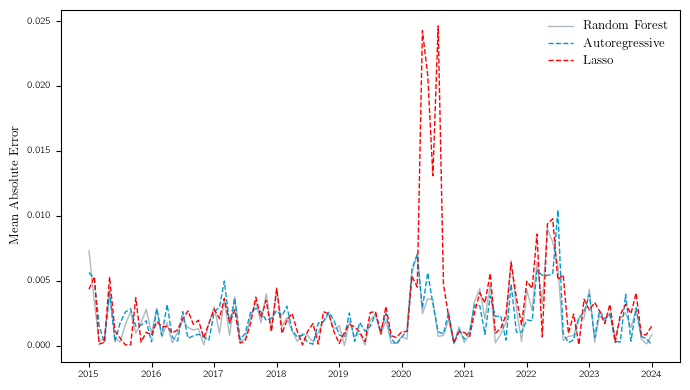
\includegraphics[width=1\linewidth]{figures/errors.png}
    \vspace{-30pt}
    \caption{Mean Absolute Error of CPI Forecasts, by Model.}
    \label{fig:errors} 
\end{figure}


Taking the relevant periods in turn, I turn first to the pre-Covid period, January 2015–January 2020. The errors for this period are shown in Table \ref{tab:errors_pre}. The models exhibit notably lower error metrics, reflecting the predictable nature of inflation trends absent significant shocks. Consistent with the finding in the literature, the RF model shows superior performance with the lowest RMSE of 0.002114 and MAE of 0.001641, suggesting its effective capture of underlying economic patterns during stable times. The Lasso model also performs well, closely following the RF with an RMSE of 0.002156 and MAE of 0.001725. Importantly, both models manage to beat the standard AR model, a feat that many inflation forecasts struggle with, as discussed in \S \ref{sec:lit_review}. Table \ref{tab:diff_pre} shows the percentage difference in forecast errors between the RF and other models. The RF is 4.28\% and 8.79\% better in RMSE and MAE terms, respectively, than the AR model. 



\begin{table}[H]
\centering
\caption{Forecast Errors — Pre-Covid: January 2015–January 2020} \label{tab:errors_pre}
\begin{tabular}{lcccc}
\toprule
& RW & AR & RF & Lasso \\
\midrule
RMSE & 0.002580 & 0.002209 & 0.002114 & 0.002156 \\
MAE  & 0.002098 & 0.001799 & 0.001641 & 0.001725 \\
MAD  & 0.001837 & 0.001671 & 0.001334 & 0.001424 \\
\bottomrule
\end{tabular}
\end{table}


\begin{table}[H]
\centering
\caption{Percentage Difference in Forecast Errors — Pre-Covid} \label{tab:diff_pre}
\begin{tabular}{lccc}
\toprule
Error Type & RF-AR & RF-RW & RF-Lasso \\
\midrule
RMSE & -4.28\% & -18.04\% & -1.95\% \\
MAE  & -8.79\% & -21.79\% & -4.90\% \\
MAD  & -20.16\% & -27.40\% & -6.37\% \\
\bottomrule
\end{tabular}
\end{table}


The advent of the Covid-19 pandemic saw a series of cascading shocks to inflation. Broadly speaking, the initial pandemic period saw a large negative shock to inflation as households were told to stay at home and firms closed. This was then followed by a period of rolling supply shocks, first in the form of supply chain disruptions resulting from prolonged Covid lockdowns in global manufacturing hubs, like China, and then the energy and food supply shocks caused by Russia's invasion of Ukraine in February 2022. This presents a challenge to any inflation forecasting model, as underlying relationships between variables can change quickly, in a way that can have nonlinear and chaotic effects on prices. 

Figure \ref{fig:errors_covid} shows a close-up of Figure \ref{eq:errors} for the period following the initial Covid shock (July 2020 onwards). The forecast errors for just this period are displayed in Table \ref{tab:errors_post}. During this period of upheaval, the AR model adjusts best to these conditions, exhibiting the lowest RMSE (0.003068) and MAE (0.002276) among the models, which points to its strength in adapting to more volatile economic environments. The Lasso model, however, struggles considerably during this period, with the highest RMSE and MAE (0.005705 and 0.003826, respectively). This is discussed further below in \S \ref{sec:analysis_lasso}. 


\begin{figure}[H]
    \centering
    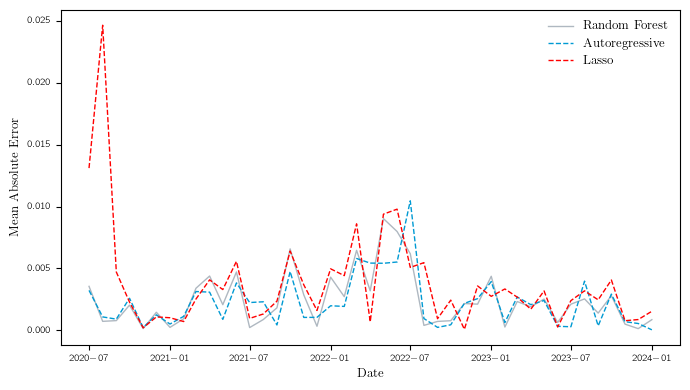
\includegraphics[width=1\linewidth]{figures/errors_covid.png}
    \vspace{-30pt}
    \caption{Mean Absolute Error of CPI Forecasts, by Model, Since Covid.}
    \label{fig:errors_covid} 
\end{figure}



\begin{table}[H]
\centering
\caption{Forecast Errors — Recent Shocks: July 2020–January 2024} \label{tab:errors_post}
\begin{tabular}{lcccc}
\toprule
& RW & AR & RF & Lasso \\
\midrule
RMSE & 0.003629 & 0.003068 & 0.003284 & 0.005705 \\
MAE  & 0.002697 & 0.002276 & 0.002462 & 0.003826 \\
MAD  & 0.002148 & 0.001940 & 0.001994 & 0.002642 \\
\bottomrule
\end{tabular}
\end{table}



Looking at the whole period (January 2015–January 2024), Table \ref{tab:errors_whole} shows that the AR model exhibits a slightly superior performance with the lowest RMSE (0.002750) compared to the RF's RMSE of 0.002766, suggesting its robustness over varied economic cycles. However, it is notable that the RF model shows a better MAE (0.002058) than the AR model (0.002102), indicating its consistency in minimising larger errors across predictions. The Lasso model again shows the least favourable performance (RMSE of 0.005026 and MAE of 0.002984), reinforcing the challenges it faces in periods marked by significant economic disruptions.


\begin{table}[H]
\centering
\caption{Forecast Errors — Whole Period: January 2015–January 2024} \label{tab:errors_whole}
\begin{tabular}{lcccc}
\toprule
& RW & AR & RF & Lasso \\
\midrule
RMSE & 0.003177 & 0.002750 & 0.002766 & 0.005026 \\
MAE  & 0.002437 & 0.002102 & 0.002058 & 0.002984 \\
MAD  & 0.001970 & 0.001758 & 0.001606 & 0.001792 \\
\bottomrule
\end{tabular}
\end{table}


\begin{table}[H]
\centering
\caption{Percentage Difference in Forecast Errors — Whole Series} \label{tab:diff_whole}
\begin{tabular}{lccc}
\toprule
Error Type & RF-AR & RF-RW & RF-Lasso \\
\midrule
RMSE & 0.57\% & -12.95\% & -44.97\% \\
MAE  & -2.10\% & -15.53\% & -31.01\% \\
MAD  & -8.67\% & -18.48\% & -10.39\% \\
\bottomrule
\end{tabular}
\end{table}



The relative performance of the forecasting models over different periods can be attributed to their inherent methodological differences and how these interact with the underlying economic dynamics. The RF model's strong performance in periods of economic stability is likely due to its ability to capture complex interactions between multiple economic indicators without prior assumptions about their relationships. RF, being ensemble methods, build multiple decision trees and aggregate their predictions, thereby reducing the model's variance without a substantial increase in bias. This characteristic makes them robust to overfitting, particularly useful in handling high-dimensional data common in economic datasets. However, during periods of sudden economic shocks, the RF model may not react as swiftly to structural breaks or non-linear shifts as models specifically designed to handle time-series data, like AR models.

By comparison, the AR model avoids having to capture these step-changes by just following patterns from previous time points as inputs to predict future values, inherently accounting for time-based trends and cycles. This temporal sensitivity makes AR models particularly effective in rapidly changing environments, where past values contain predictive signals about future conditions. Their ability to quickly incorporate new information as it becomes available helps explain their superior performance during economic upheavals, such as those induced by the Covid-19 pandemic.

Lasso’s performance, particularly the challenge it faced during periods of economic shocks, may be explained by the model's linear nature and its regularisation process, which tends to shrink the coefficients of less important variables towards zero. While this characteristic is beneficial for reducing complexity and avoiding overfitting by eliminating weakly contributing variables, it can also lead to underfitting in scenarios where relationships between variables become non-linear or where sudden changes in economic conditions alter these relationships fundamentally. Lasso's limitations in handling non-linear interactions can severely restrict its effectiveness under dramatic economic shifts.

Some researchers have argued that Lasso, and more broadly other regularisation techniques, can't beat normal factor models because the factor models are already, in effect, regularised models, with the relevant features included \autocite{GouletCoulombe2022HowForecasting}. One other explanation is that the Lasso model here does not allow for any nonlinearities, despite the fact that we know they play an important role in understanding macroeconomic dynamics \autocite{Forbes2022LowWorld}.

Incorporating nonlinearities into a large Lasso model is however computationally intensive, and I have not sought to address this issue comprehensively in this paper. By way of illustration, I did not have the computational resources to successfully solve a Lasso model with full nonlinearities. To make such a model tractable, I ran a demonstration model that incorporated 2nd degree polynomials and further dimensionality reduction through PCA. This included a feature selection process that generates polynomial and interaction terms up to the second degree. The tentative results are included for reference in the Appendix at Table \ref{tab:appendixlasso}. It indicates that the performance of the Lasso can be improved, while remaining tractable, by introducing nonlinearities in a constrained way.

\subsection{Feature Importance — Unpacking the Lasso} \label{sec:analysis_lasso}

While Lasso's forecasting performance was less impressive during the post-Covid shock period, it offers distinct advantages, especially when it comes to understanding the importance of different features. Unlike methods such as RF, which is a non-linear model that can handle complex interactions between features but does not inherently provide straightforward interpretability regarding the importance of each feature, Lasso imposes sparsity on the coefficient estimates. This property of Lasso is crucial in high-dimensional datasets where the number of predictors can be large compared to the number of observations.

The Lasso achieves this by penalising the sum of the absolute values of the regression coefficients, as encapsulated in the regularisation term $\lambda \sum_{j=1}^p |\beta_j|$. This penalty term not only helps in avoiding overfitting but also shrinks the less important feature's coefficients exactly to zero, thus performing feature selection automatically. This aspect of Lasso is particularly beneficial in inflation forecasting, where economists are often interested in identifying which variables (such as interest rates, unemployment figures, or manufacturing indexes) most significantly impact inflation. The Lasso method, therefore, not only simplifies the model but also enhances its interpretability by clearly delineating which features are most predictive of inflation, enabling policymakers and economists to focus on these key indicators.

Table \ref{tab:lasso} contains the average number of zero coefficients, the average number of non-zero coefficients, and the top 10 predictors with the highest average absolute values of their coefficients, indicating the strength and importance of each in the model's forecasting ability, across all iterations of the Lasso model.

A high number of zero coefficients (421.30 on average) indicates that the Lasso model found a substantial number of the predictors to be irrelevant or redundant when forecasting inflation. This is indicative of a sparse model, where only a small subset of the available predictors is used, reducing the risk of overfitting and improving model interpretability. Relatedly, there was an average of 34.81 non-zero coefficients, suggesting that while the model simplifies by eliminating many predictors, it still relies on a core set of features to make forecasts. These features are deemed by the model to have substantial influences on the movements in inflation.

The feature list is interesting because it shows a series of variables theory tells us are important in determining inflation also determine it empirically. The Federal Funds Rate (`FEDFUNDS'), used as both the 1-month and 4-month lagged predictors, stands out with coefficient values of 0.000179 and 0.000265, respectively.\footnote{Note, the values are displayed as absolute values. The actual `FEDFUNDS' coefficient was negative, as we would expect.} This underscores the importance of interest rate changes in forecasting inflation trends. The reserves of depository institutions (`NONBORRES'), which we can think of as forming part of the credit and banking channels of monetary policy, and average weekly hours (`AWHMAN'), as the Phillips curve term \autocite{Phillips1958The186119571}, also emerge as significant predictors, with coefficients across multiple lags. Other variables theory tells us are important in the transmission of monetary policy were also significant in determining inflation. Treasury spreads and yields, as reflected by `TB3SMFFM', `GS5', and `GS10', play a significant role, highlighting the impact of short and long-term interest rate movements on inflationary expectations. The coefficients associated with these features suggest that shifts in the yield curve contain important information for forecasting inflation.


\begin{table}[H]
\centering
\caption{Lasso Model Summary Statistics and Top 10 Most Important Features} \label{tab:lasso}
\begin{tabular}{lcr}
\toprule
Statistic & Value & \\
\midrule
Average Number of Zero Coefficients & 421.30 & \\
Average Number of Non-Zero Coefficients & 34.81 & \\
\midrule
\multicolumn{3}{c}{Top 10 Most Important Features} \\
\midrule
Feature & Coefficient & Lag \\
\midrule
FEDFUNDS & 0.000265 & 4 \\
NONBORRES & 0.000206 & 4 \\
AWHMAN & 0.000179 & 1 \\
FEDFUNDS & 0.000179 & 1 \\
NONBORRES & 0.000146 & 3 \\
BAAFFM & 0.000128 & 2 \\
TB3SMFFM & 0.000119 & 4 \\
GS5 & 0.000118 & 1 \\
GS10 & 0.000092 & 4 \\
AWHMAN & 0.000085 & 4 \\
\bottomrule
\end{tabular}
\end{table}

